% Compact dissertation based on the reviewed 18 November 2026 WKU source.
\documentclass[12pt,a4paper,oneside]{report}
\usepackage[T1]{fontenc}
\usepackage[utf8]{inputenc}
\usepackage{lmodern}
\usepackage[nopatch=footnote]{microtype}
\usepackage[top=1in,bottom=0.689in,hmargin=1.25in,nohead,includefoot,foot=0.311in,footskip=0.5827in]{geometry}
\usepackage{amsmath,amssymb,amsthm,mathtools,mathrsfs}
\usepackage{booktabs,array,tabularx,longtable}
\renewcommand{\tabularxcolumn}[1]{>{\raggedright\arraybackslash}p{#1}}
\usepackage{graphicx,tikz,pgfplots,pgfplotstable,adjustbox}
\BeforeBeginEnvironment{tikzpicture}{\begin{adjustbox}{max width=\linewidth}}
\AfterEndEnvironment{tikzpicture}{\end{adjustbox}}
\usetikzlibrary{arrows.meta,positioning,calc}
\usepgfplotslibrary{groupplots}
\pgfplotsset{compat=1.18}
\usepackage[numbers,sort&compress]{natbib}
\usepackage[hyphens]{url}
\usepackage{hyperref,bookmark}
\usepackage{setspace,fancyhdr,titlesec,caption,placeins}
\definecolor{ink}{HTML}{263B5E}
\definecolor{teal}{HTML}{087F8C}
\definecolor{warm}{HTML}{B65528}
\definecolor{keyred}{HTML}{AB2634}
\definecolor{reviewblue}{HTML}{144F9C}
\newcommand{\keyeq}[1]{\textcolor{keyred}{#1}}
\newcommand{\reviewnote}[1]{\textcolor{reviewblue}{\textit{Revision: #1}}}
\hypersetup{colorlinks=true,linkcolor=ink,citecolor=teal,urlcolor=teal,
 pdfauthor={Yihong Xiao},
 pdftitle={Parameter-Dependent Lie Symmetries and Semi-Analytical Solutions of Nonlinear PDEs},
 pdfsubject={Undergraduate dissertation, MATH 4890}}
\titleformat{\chapter}[hang]{\normalfont\Large\bfseries\raggedright}{\thechapter.}{.7em}{}
\titlespacing*{\chapter}{0pt}{-20pt}{12pt}
\titleformat{\section}{\normalfont\large\bfseries}{\thesection}{.6em}{}
\titlespacing*{\section}{0pt}{8pt plus 2pt}{3pt}
\titlespacing*{\subsection}{0pt}{8pt plus 2pt}{3pt}
\captionsetup{font=small,labelfont=bf,skip=4pt}
\setlength{\textfloatsep}{10pt plus 2pt minus 2pt}
\setlength{\intextsep}{9pt plus 2pt minus 2pt}
\renewcommand{\topfraction}{.9}
\renewcommand{\textfraction}{.08}
\setstretch{1.0}
\setlength{\emergencystretch}{2em}
\setlength{\parskip}{0pt}
\setcounter{tocdepth}{1}
\makeatletter
\renewcommand{\@pnumwidth}{2.8em}
\renewcommand{\@tocrmarg}{3.8em}
\makeatother
\raggedbottom
\numberwithin{equation}{chapter}
\newtheorem{theorem}{Theorem}[chapter]
\newtheorem{proposition}[theorem]{Proposition}
\newtheorem{corollary}[theorem]{Corollary}
\newtheorem{definition}[theorem]{Definition}
\theoremstyle{remark}\newtheorem{remark}[theorem]{Remark}
\newcommand{\dd}{\,\mathrm d}
\newcommand{\E}{\mathcal E}
\newcommand{\pr}{\operatorname{pr}}
\newcommand{\rank}{\operatorname{rank}}
\newcommand{\norm}[1]{\left\lVert#1\right\rVert}
\DeclareRobustCommand{\code}[1]{\nolinkurl{#1}}
\newcommand{\doi}[1]{\href{https://doi.org/#1}{doi: #1}}
\pagestyle{fancy}\fancyhf{}
\renewcommand{\headrulewidth}{0pt}
\fancyfoot[R]{\thepage}
\fancypagestyle{plain}{\fancyhf{}\fancyfoot[R]{\thepage}\renewcommand{\headrulewidth}{0pt}}
\setlength{\tabcolsep}{1mm}
\renewcommand{\arraystretch}{1.3}
\renewcommand{\bibname}{References}
\renewcommand{\chaptermark}[1]{\markboth{\thechapter.\ #1}{}}
\tikzset{box/.style={draw=ink,fill=ink!4,rounded corners=2pt,
 align=center,inner sep=5pt,font=\small},
 planned/.style={box,draw=teal,fill=teal!5,dashed},
 arr/.style={-{Latex[length=2mm]},thick,ink},
 warnbox/.style={draw=warm,fill=warm!5,rounded corners=2pt,align=center,inner sep=4pt,font=\scriptsize},
 mlbox/.style={draw=teal,fill=teal!6,rounded corners=2pt,align=center,inner sep=4pt,font=\scriptsize},
 note/.style={font=\scriptsize,align=center},
 warr/.style={-{Latex[length=1.8mm]},thick,warm,dashed},
 tarr/.style={-{Latex[length=1.8mm]},thick,teal}}

\begin{document}
\hypersetup{pageanchor=false}
\pagenumbering{Roman}
\begin{titlepage}
\thispagestyle{plain}
\noindent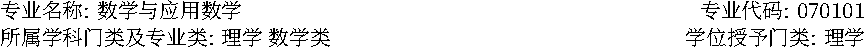
\includegraphics[width=\textwidth]{wku_programme_header.pdf}
\vspace{18mm}
\begin{center}
\textbf{College of Science, Mathematics and Technology}\par
\medskip
\textbf{Wenzhou-Kean University}\par
\vspace{8mm}

\includegraphics[width=2.2055in,height=1.9055in]{WKU.png}\par
\vspace{25mm}
{\bfseries Parameter-Dependent Lie Symmetries\par
and Semi-Analytical Solutions\par
of Nonlinear PDEs\par}
\vspace{4mm}
Saint--Venant--Exner Case Studies\par
{\small Lie-Invariant Reference Families and Targeted Corrections\par}
\vspace{3mm}
Undergraduate Dissertation (MATH 4890)
\end{center}
\vspace{10mm}
\noindent\begin{tabularx}{\textwidth}{@{}lX@{}}
\textbf{Student Name:} & \underline{Yihong Xiao}\\[4pt]
\textbf{Student ID:} & \underline{1308225}\\[4pt]
\textbf{Major:} & \underline{Mathematical Sciences}\\[-2pt]
 & \underline{(Data Analytics Option)}\\[4pt]
\textbf{Supervisor:} & \underline{Dr.\ Puneet Rana}\\[4pt]
\textbf{Date of Submission:} & \underline{11 November 2026}
\end{tabularx}
\end{titlepage}
\hypersetup{pageanchor=true}
\setcounter{page}{2}
\chapter*{Author's Declaration}
\addcontentsline{toc}{chapter}{Author's Declaration}
I, the undersigned, hereby declare that this submission is entirely my own work, in my own words, and that all sources used in researching it are fully acknowledged and all quotations properly identified. It has not been submitted, in whole or in part, by me or another person, for the purpose of obtaining any other credit/grade. I have a citation to AI system used to generate the text if I used AI-generated text. I understand the ethical implications of my research, and this work meets the requirements of College of Science, Mathematics and Technology.

\vspace{25mm}
\noindent\textbf{Date:} \rule[-8pt]{11.5cm}{0.1em}\par
\bigskip\bigskip
\noindent\textbf{Name (printed letters):} \rule[-8pt]{7.8cm}{0.1em}\par
\bigskip\bigskip
\noindent\textbf{Signature:} \rule[-8pt]{10.55cm}{0.1em}
\vfill
{\small\noindent\textit{AI assistance disclosure.} OpenAI ChatGPT assisted with
drafting, compression, mathematical exposition, verification code, and
typesetting in November 2026. See \url{https://chatgpt.com/}. The declaration
above remains unsigned for the author's review.}
\clearpage
\chapter*{Abstract}
\addcontentsline{toc}{chapter}{Abstract}
\noindent\textbf{Goal.} Determine how parameter-dependent Lie symmetries and singular branches of Saint--Venant--Exner equations provide physically reconstructible reference solutions for specified nearby problems.

\medskip\noindent\textbf{Method.} Verify prolonged actions in jet coordinates, derive invariant graphs and restrict the equations to regular quotient charts. Compare the printed scalar $P$ and the material scalar $M$ on a shared quotient. Lift the profiles to the original fields and independently check the balances. Compare exact, series, numerical and learned profiles on declared data.

\medskip\noindent\textbf{Result.} On their stated local charts, the analysis gives material reconstruction, an exact travelling wave, a convergent cubic Laurent branch and two analytic crossing germs at a compatible saddle of the separate annular model. On the positive charts the point symmetries of $E_1$, $P$ and $M$ are classified for real $m\ge1$. Chebyshev collocation gives smaller sampled field errors than the liquid-block model on the controlled benchmarks. \reviewnote{Classify the remaining singular profiles and planar symmetries before extending the scope. A matched-accuracy cost claim requires a paired correction test.}

\medskip\noindent\textbf{Keywords} \quad Parameter-dependent Lie symmetries, jet bundles, invariant reduction, Saint--Venant--Exner system, material reconstruction, singular branches, Laurent series, structure-constrained neural approximation.
\clearpage
\tableofcontents
\clearpage
\addcontentsline{toc}{chapter}{List of Figures}
\listoffigures
\clearpage
\addcontentsline{toc}{chapter}{List of Tables}
\listoftables
\clearpage
\chapter*{List of Symbols and Abbreviations}\label{sec:notation}
\addcontentsline{toc}{chapter}{List of Symbols and Abbreviations}
\noindent\begin{tabularx}{\textwidth}{@{}p{.25\textwidth}X@{}}
\toprule
Symbol & Meaning and dimension \\\midrule
$E_1,E_2,E_{\rm exch}$ & One-dimensional Eulerian system, rotating planar system, and a separate planar exchange extension.\\
$P,M$ & Printed and compatible scalar equations on the material chart, respectively.\\
$t,x,y,s$ & Time, Cartesian positions, and material mass coordinate. Dimensional units are given in Chapter~\ref{ch:models}.\\
$h,u,B,\mathbf w,a$ & Water depth, one-dimensional velocity, bed elevation or thickness, planar velocity, and mobile chemical load. The planar velocity has two components.\\
$g,\kappa,m$ & Gravity coefficient, scalar bedload coefficient and dimensionless bedload exponent.\\
$X,\pr^{(n)}X,Q_X$ & Point generator, its action on derivatives through order $n$, and its invariant-surface characteristic.\\
$z,\sigma,F$ & Scalar invariant coordinates and their scalar profile. A prime denotes differentiation in the active profile coordinate.\\
$r,H,V,W,Z$ & Radius, depth, radial velocity, azimuthal velocity, and bed profile for the annular reduction.\\
$P_Z,D,N$ & Recovered bed slope, leading radial coefficient, and right-hand side of the undivided radial equation $DH'=N$.\\
$\vartheta,\theta$ & Equation or trace parameters, and fitted approximation coefficients, respectively.\\
\bottomrule
\end{tabularx}
\clearpage
\pagenumbering{arabic}

\chapter{Introduction}\label{ch:introduction}
Shallow water moving over a mobile bed transports both water and sediment. Flow changes the bed through its sediment flux. In turn, the bed slope changes the pressure force on the flow. Lie symmetry gives a way to derive lower-dimensional equations for selected solutions of this coupled system \cite{fernandez2017,olver,oliveri}. The central question here is whether a verified invariant family can provide a useful reference for computing solutions of a specified nearby problem.

Three issues determine the answer. First, parameters can change the admitted generator class and the regularity of constitutive terms. Second, the base orbit rank and transversality determine which variables a reduction can remove. Third, reduced coefficients can vanish, requiring a different analytic chart even when the symmetry action remains regular. These issues concern the equation and its data. A change of the sediment exponent alone does not describe every change of model.

The analysis uses four outcomes with different hypotheses. An invariant reference follows from a verified substitution and reconstruction. An analytic approximation additionally needs convergence and derivative bounds. A proposed correction must solve a changed problem with explicit data. A validated correction also needs a stability estimate. Numerical evidence in Chapter~\ref{ch:computation} compares restricted profiles. The broader function-space correction remains conditional.

\begin{figure}[htb]\centering
\begin{tikzpicture}[x=1cm,y=1cm]
\node[box,text width=2.75cm] (a) at (0,0) {Equations, closure\\and data};
\node[box,text width=2.75cm] (b) at (3.65,0) {Prolongation\\and transverse orbits};
\node[box,text width=2.75cm] (c) at (7.30,0) {Quotient equation\\and analytic branch};
\node[box,text width=2.75cm] (d) at (10.95,0) {Reconstruction\\and original residual};
\draw[arr] (a)--(b); \draw[arr] (b)--(c); \draw[arr] (c)--(d);
\node[planned,text width=5.5cm] (e) at (8.8,-1.55) {Changed parameters or data \quad $\longrightarrow$ \quad targeted correction and stability check};
\draw[tarr] (d.south) |- (e.east);
\end{tikzpicture}
\caption[Reduction and reconstruction workflow]{The number of remaining independent variables is fixed by the selected base orbit rank. The reconstructed reference may then be used in a separate target problem.}
\label{fig:workflow}
\end{figure}

\chapter{Physical Model and Material Reconstruction}\label{ch:models}
\section{Eulerian water and bed equations}
Let $L_0,H_0,U_0$ be positive reference scales for horizontal position, depth, and velocity, and set $T_0=L_0/U_0$. In dimensional coordinates $x$ has units of length, $t$ of time, $h,B$ of length, $u$ of length per time, and sediment flux $q$ of length squared per time. The mass coordinate $s$ has scale $H_0L_0$. We work with dimensionless variables unless units are stated, with $g$ denoting dimensional gravity times $H_0/U_0^2$. A comparison across exponents keeps the reference scales fixed.

The one-dimensional Eulerian model $E_1$ uses $(h,u,B)(t,x)$ on $h,u>0$:
\begin{align}\label{eq:E}
 \Delta_h&=h_t+(hu)_x=0,\qquad
 \Delta_u=u_t+uu_x+g(h+B)_x=0,\notag\\
 \Delta_B&=B_t+\kappa(u^m)_x=0 .
\end{align}
Here $m\ge1$ and $\kappa=A_g/(1-\epsilon_{\rm bed})>0$ combines the transport coefficient and porosity. The momentum balance printed in the 2022 paper is in conservative variables. Its residual is $h\Delta_u+u\Delta_h$, so the two forms agree on this chart \cite{sve2022}. A bed-slope flux $-G_0u^n B_x$ can be incorporated by replacing $q=\kappa u^m$ by $q=\kappa u^m-G_0u^n B_x$. Equations and results using $q=\kappa u^m$ keep that closure.


For a dimensional flux $q=A_g u^m/(1-\epsilon_{\rm bed})$, the dimensions of
$A_g$ are length$^{2-m}$ time$^{m-1}$. Keeping the numerical value of a
dimensional coefficient fixed while changing $m$ therefore need not describe
the same constitutive comparison. The power law is real analytic on $u>0$.
At $u=0$, regularity depends on the exponent and on the chosen extension to
negative velocities.

\section{The printed scalar and a compatible scalar}
Continuity makes $h\,dx-hu\,dt$ closed. On a small chart take $s_x=h$, $s_t=-hu$ and invert to $x=\phi(t,s)$. Put $b(t,s)=B(t,\phi(t,s))$. Then
\begin{equation}\label{eq:chain}
 \phi_s=1/h,\quad \phi_t=u,\qquad
 \partial_x=\phi_s^{-1}D_s,\quad
 \partial_t\big|_x=D_t-\frac{\phi_t}{\phi_s}D_s .
\end{equation}
Here $D_t,D_s$ differentiate composites in material coordinates. Define
\[
 A=\phi_s\phi_{tt}-g\phi_{ss}/\phi_s^2,\qquad
 T_m=\phi_t^{m-1}\phi_{ts}/\phi_s,\qquad \beta=m\kappa .
\]
The material balances are $A+gb_s=0$ and
$b_t-(\phi_t/\phi_s)b_s+\beta T_m=0$. Their compatibility equation is $M$. Equation (7) of the 2026 source defines a separate reproduction target $P$ \cite{ap}:
\begin{align}
 P[\phi]&=D_t A-g\beta D_s T_m,\label{eq:P}\\
 \keyeq{M[\phi]}&\keyeq{{}=P[\phi]-D_s\!\left(\frac{\phi_t}{\phi_s}A\right).}\label{eq:M}
\end{align}
The last term comes from differentiating the bed at a fixed Eulerian position. For example, $\phi=t+s+s^3/6$ has $P[\phi]=0$, while $M[\phi]=8g(2-5s^2)/(2+s^2)^4$ equals $g$ at $s=0$.

\begin{proposition}[Local physical reconstruction]\label{prop:material}
On a simply connected material chart with $\phi_s,\phi_t>0$, a sufficiently smooth $M$ solution determines a bed, unique up to a constant, by
\begin{equation}\label{eq:bed-form}
 \keyeq{db=-\frac{A}{g}\,ds-\left(\frac{\phi_t A}{g\phi_s}+\beta T_m\right)dt.}
\end{equation}
On each small chart where $x=\phi(t,s)$ is invertible, the fields $h=1/\phi_s$, $u=\phi_t$, $B=b$, composed with the inverse, solve $E_1$.
\end{proposition}
\begin{proof}
The form is closed by~\eqref{eq:M}, so it has a primitive and recovers the two material balances. For continuity, the time derivative of $1/\phi_s$ in~\eqref{eq:chain} is
$-\phi_{ts}/\phi_s^2+\phi_t\phi_{ss}/\phi_s^3$, which cancels $\phi_s^{-1}D_s(\phi_t/\phi_s)$. The inverse function theorem applies since $\phi_s>0$. On a sufficiently small rectangle, each fixed-time map is strictly increasing. This is a local solution correspondence.
\end{proof}


\begin{figure}[htb]\centering
\begin{tikzpicture}[x=1cm,y=1cm]
\node[box,text width=5.35cm] (e) at (0,0) {\textbf{Eulerian balance $E_1$}\\Water and bed fields at fixed positions};
\node[box,text width=5.35cm] (l) at (6.65,0) {\textbf{Coupled material balances}\\Particle map and advected bed};
\node[warnbox,text width=5.35cm] (p) at (0,-1.65) {\textbf{Printed scalar equation $P$}\\Separate reproduction target};
\node[box,text width=5.35cm] (m) at (6.65,-1.65) {\textbf{Compatible scalar equation $M$}\\Local recovery by the closed bed form};
\draw[Latex-Latex,ink,thick] (e)--(l);
\draw[Latex-Latex,ink,thick] (l)--(m);
\draw[gray,densely dashed] (p)--(m) node[midway,above,warm,font=\small] {$P\ne M$};
\end{tikzpicture}
\caption[Three water and sediment descriptions]{The two local equivalences use the invertible chart and the bed gauge of Proposition~\ref{prop:material}. The scalar reproduction target has a different residual.}
\label{fig:material-chart}
\end{figure}

\chapter{Lie Reduction and Reproduction Checks}\label{ch:lie}
\section{Prolongation, quotient and solvable coordinates}
Let $U$ have $q$ components on a $d$-dimensional base including time. The $n$th jet space records the independent coordinates, field values and derivatives through order $n$. A regular system $\Delta=0$ defines a submanifold of this space. For a point field $X=\xi^i\partial_{x^i}+\eta^a\partial_{U^a}$, define
\[
 Q_X^a=\eta^a-\xi^iU_i^a,\qquad
 \eta^a_{J,i}=D_i\eta^a_J-(D_i\xi^j)U_{J,j}^a,\qquad \eta^a_\varnothing=\eta^a .
\]
Here repeated component indices are summed and $J$ is a derivative multi-index. The recursion follows by differentiating transformed graphs. Tangency of $\pr^{(n)}X$ to $\Delta=0$ verifies an infinitesimal symmetry on the regular jet chart. Differential consequences must be included when eliminating derivatives \cite[Chs.~2--3]{olver} and \cite{oliveri}. Orbit weights also establish tangency when all terms of each equation scale together.

For a selected Lie subalgebra whose point orbits and projected base orbits both have rank $k$, assume local quotients exist and use a chart transverse to the base orbits. Invariant graphs satisfy $Q_X=0$ for its generators. In adapted coordinates each graph then depends on $d-k$ base invariants. To see the local correspondence, restrict each invariant graph to a transverse section, then take the union of its orbits. Equal ranks and the section hypothesis make this lift locally single-valued. Substitute the lift into the original equations. Invariance of the equation locus extends the vanishing residual off the section within that chart. Singular strata, graphs with different isotropy, and domain or boundary data require their own checks \cite{anderson2000}. A vertical translation of a field can preserve the equation while $Q_X=1$ rules out invariant graphs for that generator.

For a projectable subgroup $H$, let $B_0$ denote the base and $\bar E\to B_0/H$ the reduced bundle on a regular transverse chart. A reduced section determines a local invariant lift. Pull the original residual back by the jet map of that lift. The invariant equations are $\keyeq{Q_X=0}$ for $X\in\mathfrak h$. A generator in the normalizer of $\mathfrak h$ preserves its orbit foliation, so $N_{\mathfrak g}(\mathfrak h)/\mathfrak h$ supplies the inherited infinitesimal action, possibly with a kernel. For the cubic scaling, $\partial_\phi$ commutes with $X_5$ and descends to $\partial_F$. The common-scaling first integral follows directly from the residual identity below.


\section{Parameter dependence of generators}
In a declared finite class with analytic determining matrix $A(\mu)$, any fixed-rank analytic parameter chart gives a local analytic basis for $\ker A(\mu)$. A nonzero maximal minor solves pivot coordinates in terms of the free coordinates. At a rank jump extra directions can exist only at the exceptional value, as shown by $\mu a=0$. For a differentiable family of generators through $X_0$ in a fixed determining space, the directional derivative $X_1$ must satisfy
\begin{equation}\label{eq:continue}
 \mathscr D_{\mu_0} X_1=-(\partial_\nu\mathscr D)_{\mu_0}X_0.
\end{equation}
This follows by differentiating the determining identity. An obstruction follows if a linear functional annihilates the whole range of $\mathscr D_{\mu_0}$ in the proposed correction class and is nonzero on the right. A finite search or a test against only diagonal fields cannot prove this for all point fields \cite{dengreid2024}. Similarly, a space of actual analytic symmetry germs is finite dimensional exactly when some finite jet map is injective on it: the descending jet kernels stabilize in finite dimension and have zero intersection by analyticity. Formal jet kernels alone give no realization argument.

On the positive chart $p=\phi_t>0$, $q=\phi_s>0$, the unrestricted smooth point algebras of $P$ and $M$ have the common basis $\partial_t,\partial_s,\partial_\phi,t\partial_t+s\partial_s+\phi\partial_\phi$. At $m=3$ both admit the additional $X_5=t\partial_t-2s\partial_s$. At $m=1$ only $P$ admits $t\partial_\phi$. Its finite defect on $M$ is $-\varepsilon D_s(A/\phi_s)$.

For $M$, start with arbitrary functions $\tau,\xi,\eta$ of $(t,s,\phi)$. Solve the equation for $\phi_{ttt}$ using its coefficient $q$ and restrict the determining identity to zero second jets. The coefficient of the free $\phi_{tts}$ jet, multiplied by $q^4$, splits in $q$ and $p$. Its highest and lowest powers give $\xi_t=\xi_\phi=\tau_s=0$. The two middle coefficients give $\tau_\phi=\eta_s=\eta_t=0$. The free $\phi_{tss}$ coefficient then gives
\[
 3\eta_\phi=\xi_s+2\tau_t,\qquad (m-3)(\eta_\phi-\tau_t)=0 .
\]
The three derivatives depend on separate variables and are constant. The full prolongation verifies the resulting generators. The companion calculation for $P$ also splits unrestricted coefficients and retains the time-linear $\phi$ translation at $m=1$. Exact checks and connected one-dimensional adjoint representatives for every parameter stratum are in the final delivery code and verification record.


\section{The 2022 and 2026 equations}
For $E_1$ with positive transport and positive depth and velocity, the unrestricted first-order determining system gives time and space translations, simultaneous time and space dilation, and a bed shift for every real $m\ge1$. The proof separates $m=1$ before using the derivative of the transport coefficient, which is positive on $m>1$. At $m=3$ a further verified generator is
\[
 X_5=t\partial_t-u\partial_u-2h\partial_h-2B\partial_B .
\]
Its prolongation on the bed balance, restricted to $\Delta_B=0$, is $(3-m)\kappa(u^m)_x$. The water balances have common weights separately for each equation. Substitution of the coefficients in printed equation (25) gives a nonzero continuity defect $-(hu)_x$ on shell. Using the verified $X_5$, the invariant graph on $t>0$ is $(u,h,B)=(U(x)/t,H(x)/t^2,Z(x)/t^2)$. Its profile equations are
\[
 (HU)'=2H,\qquad UU'-U+g(H'+Z')=0,\qquad \kappa(U^3)'=2Z .
\]
They admit $U=2x/3$, $H=(1-4g\kappa)x^2/(9g)$, $Z=4\kappa x^2/9$ on $x>0$, $4g\kappa<1$. The printed scaling and this corrected solution are checked by explicit residual substitution. The full catalogue of published representatives and rejected formulas is retained in the project reproduction notes. These checks concern selected generators and solutions.

For $P$ at $m=3$, use $X=t\partial_t-2s\partial_s$. Its flow yields $t\mapsto e^a t$, $s\mapsto e^{-2a}s$, $\phi\mapsto\phi$. The invariant variables $\sigma=st^2$ and $\phi$ give $\phi=F(\sigma)$ on $t>0$. With $p=F'>0$, the substituted expressions are $A=A_\sigma$ and $T_3=t^{-3}J_\sigma$, where
\begin{equation}\label{eq:cubic-terms}
 A_\sigma=2\sigma p^2+4\sigma^2pp'-gp'/p^2,qquad
 J_\sigma=8\sigma^2 p(p+\sigma p').
\end{equation}
Thus
\begin{equation}\label{eq:cubic-reduced}
 tP[F]=2\sigma A_\sigma'-g\beta J_\sigma',\qquad
 -t M[F]/2=A_\sigma+\tfrac12g\beta J_\sigma' .
\end{equation}
The factor $t$ removed from $P$ is nonzero. The reduced third-order equation has one independent variable, even though its reconstructed solution evolves with $t$. The second identity uses the extra term $-2t^{-1}(\sigma A_\sigma)'$ from~\eqref{eq:M}; it will be used for the physical Laurent branch.


A simpler Eulerian reference follows from the symmetry
$\partial_t+\alpha\partial_B$. Its invariant graph has $h=H(x)$, $u=U(x)$,
$B=\alpha t+Z(x)$. Integrating the reduced continuity and sediment balances
gives $HU=A_1$ and $U^m=A_2-\alpha x/\kappa$. On the positive branch,
the primitive momentum equation is the derivative of
$U^2/2+g(H+Z)=A_3$. Thus $Z=A_3/g-H-U^2/(2g)$, which supplies the first
comparison case below. The time dependence of the bed survives the lift
as the known drift $\alpha t$.

\section{An exact physically reconstructed travelling wave}
A different verified symmetry of $M$ is $\partial_t+c\partial_s$, with $c<0$. Its invariant graph is $\phi=F(z)$, $z=s-ct$. Setting $p=F'>0$ in~\eqref{eq:M} gives $M[F]=g\beta c(-c)^{m-1}(p^{m-2}p')'$. After integration,
\[
 p^{m-2}p'=k,\qquad F'=p.
\]
At $m=1$, $p=p_*e^{k(z-z_*)}$ and
$F=F_*+p_*(e^{k(z-z_*)}-1)/k$ for $k\ne0$. At $k=0$ this is affine. At $m>1$, $p^{m-1}=p_*^{m-1}+(m-1)k(z-z_*)$ on its positive interval. Quadrature gives $F$, and~\eqref{eq:bed-form} gives
\[
 x=F(s-ct),\quad h=1/p,\quad u=-cp,\quad
 b=b_0-1/p-c^2p^2/(2g)+\beta c(-c)^{m-1}kt .
\]
These fields solve all of $E_1$ locally. Introducing $p=F'$ reduces derivative order using the profile translation symmetry. The invariant-graph requirement concerns the earlier reduction in independent variables.

\chapter{Singularity-Adapted Analytic Profiles}\label{ch:series}
\section{First integrals and the leading coefficient}
The joint dilation $t\partial_t+s\partial_s+\phi\partial_\phi$ acts on $P$ and $M$ with residual weight $-2$. Its invariant graph on $t>0$ is $\phi=tF(z)$ with $z=s/t$. Put $p=F'$, $V=F-zp$, and require $p,V>0$. In this section $V$ is the material velocity. Substituting $A=F''(z^2p-g/p^2)/t$ and $T_m=-zV^{m-1}F''/(tp)$ gives
\begin{align}
 t^2P[tF]&=(L_P F'')', & L_P&=-z^3p+gz/p^2+g\beta zV^{m-1}/p,\label{eq:Lp}\\
 \keyeq{t^2M[tF]}&\keyeq{{}=(L_M F'')'}, & L_M&=F(g/p^3-z^2)+g\beta zV^{m-1}/p.\label{eq:Lc}
\end{align}
For the common normalization $\mathcal R_A=t^2 A[tF]$ with $A=P,M$, subtraction gives
\[
\keyeq{\mathcal R_M-\mathcal R_P
 =\frac{d}{dz}\left[V\left(\frac{g}{p^3}-z^2\right)F''\right].}
\]
The two operators share a quotient chart. This identity expresses the fixed-position bed transport contribution in that chart.
On a connected interval $\keyeq{L F''=I_0}$ for the corresponding $L$ and a constant $I_0$. At $L\ne0$, the analytic system $F'=p$, $p'=I_0/L(z,F,p)$ supplies a unique local analytic solution for prescribed $F,p,I_0$. If $F(z_0+\rho)=\sum a_j\rho^j$, then
\[
 (n+2)(n+1)a_{n+2}=[\rho^n],\frac{I_0}{L(z_0+\rho,F_{n+1},F_{n+1}')},
\]
where $F_{n+1}$ truncates at degree $n+1$ and $n\ge0$. For $M$, writing $A_*=tA$ gives the bed $b=B_*(z)+(I_0/g)\log(t/t_*)+b_0$ with $B_*'=-A_*/g$. This is a descended first integral checked through the material bed form. Point symmetry alone does not supply a conservation law \cite{druzhkov2024,noether1918}.

For $M$, the Eulerian first-order coefficient matrix is
$A_E=\left(\begin{smallmatrix} u&h&0\\g&u&g\\0&q_u&0\end{smallmatrix}\right)$.
A fixed $z$ has physical speed $F$. With $u-F=-zp$, $h=1/p$, the determinant is
$\det(A_E-FI)=p^2 L_M$. Thus $L_M=0$ expresses tangency of an orbit to an Eulerian characteristic in this chart. It is distinct from a rank jump in the determining matrix. The undivided profile equation remains meaningful there. For instance, at $m=3$, $F=A_0z^{1/3}$, $z>0$, lies on the zero-leading-coefficient branch, with $A_0^3=27g/(1-12g\kappa)$ for $P$ and $27g/(1-4g\kappa)$ for $M$, where the respective denominators are positive. These values follow by inserting the power in the corresponding $L$.

\section{A convergent cubic Laurent branch}
Use the cubic $M$ equation in~\eqref{eq:cubic-reduced}, with $t,\sigma,p>0$ on the real solution chart. A pole $F\sim-w_0/\sigma$, $w_0>0$, balances its leading terms only when $g\beta=3/4$. Set $\xi=g\sigma^4/w_0^3$, $Y=\sigma^2 F'/w_0$ and let primes on $Y$ denote $\xi$ derivatives. Then the equation becomes
\[
 3\xi Y''+3\xi(Y')^2/Y+Y'-\xi Y'/(4Y^3)+1/(8Y^2)=0 .
\]
A holomorphic branch with $Y(0)=1$ follows by iteration in the disk algebra on $|\xi|\le1/4$. Write $V=Y'$ and $Y(\xi)=1+\xi\int_0^1V(r\xi)\,dr$. The equivalent fixed-point equation is
\[
 V(\xi)=\int_0^1 r^{-2/3}\left[-\frac{1}{24Y(r\xi)^2}
   +r\xi\left(-\frac{V(r\xi)^2}{Y(r\xi)}
                +\frac{V(r\xi)}{12Y(r\xi)^3}\right)\right]dr .
\]
For $\|V\|_\infty\le1/4$ we have $\|Y-1\|\le1/16$ and $|Y|\ge15/16$. Applying those bounds, $\int_0^1 r^{-2/3}dr=3$, $\int_0^1r^{1/3}dr=3/4$, and $\|\delta Y\|\le\|\delta V\|/4$ gives an image radius below $0.160$ and a Lipschitz constant below $0.202$. Banach's theorem therefore constructs the branch. After multiplying the equation by $8Y^3$, the coefficient of $y_n$ at degree $n-1$ is $8n(3n-2)$, where $Y=\sum y_n\xi^n$. Integrating $F'$ gives
\[
 F=F_0+\frac{w_0}{\sigma}\sum_{n\ge0}\frac{y_n\xi^n}{4n-1}
   =F_0-\frac{w_0}{\sigma}-\frac{g\sigma^3}{24w_0^2}
                  -\frac{g^2\sigma^7}{512w_0^5}+O(\sigma^{11}) .
\]
The two free constants are $F_0,w_0$. For $q=4g|\sigma|^4/w_0^3<1$, Cauchy's coefficient bound $|y_n|\le (17/16)4^n$ gives
\begin{align*}
 |F-F^{[N]}|&\le\frac{17w_0}{16|\sigma|}
                 \frac{q^{N+1}}{(4N+3)(1-q)},\
 |F'-(F^{[N]})'|&\le\frac{17w_0}{16|\sigma|^2}
                 \frac{q^{N+1}}{1-q}.
\end{align*}
This establishes a sufficient punctured convergence disk and local real reconstruction for positive $\sigma$. Higher derivatives can be bounded on smaller compact annuli. The bed $b=b_0+4\beta t^{-2}\sigma^2 F'(F'+\sigma F'')$ needs a second-derivative estimate.

\section{Errors in physical coordinates}
If $\phi_s\ge\mu>0$ and $\|\widehat\phi_s-\phi_s\|_\infty\le e_s<\mu$, then on the same material labels
$|\widehat h-h|\le e_s/[\mu(\mu-e_s)]$. On a common Eulerian image, inversion additionally gives $|\widehat s-s|\le\|\widehat\phi-\phi\|_\infty/\mu$ and field Lipschitz bounds translate the label discrepancy into a field error. A smooth parameterization can isolate a pole by prescribing its principal part and learning the regular remainder. A moving pole needs its own location parameter and separate overlapping charts.

\chapter{Rotating Annular Models}\label{ch:continuation}
\section{Planar equations, rotation and radial integrals}
On a planar annulus $r=\sqrt{x^2+y^2}\in(r_0,r_1)$ with $r_0>0$, the model $E_2$ has three independent variables $(t,x,y)$ and four field components $(h,\mathbf w,B)$, where $\mathbf w=(u,v)$ and $h>0$. Put $\mathcal J(u,v)=(-v,u)$. For $g,K,G>0$ and constant $f$, work with
\begin{align}\label{eq:planar}
 h_t+\nabla\cdot(h\mathbf w)&=0,\notag\\
 \mathbf w_t+(\mathbf w\cdot\nabla)\mathbf w+g\nabla(h+B)+f\mathcal J\mathbf w&=0,\notag\\
 B_t+\nabla\cdot\mathbf Q&=0,\qquad
 \mathbf Q=|\mathbf w|^2(K\mathbf w-G\nabla B).
\end{align}
Here derivatives are planar and $\mathbf Q$ has two components. With the scales of Chapter~\ref{ch:models}, the dimensionless parameters are $f_* = f T_0$, $K_* = K U_0^2/H_0$, $G_* = G U_0/L_0$. The model treats $f$ as a constant Coriolis parameter. A centrifugal potential is explicit in the separate exchange extension below.

Translations, simultaneous position and velocity rotations, bed shifts, and the dilation $(\mathbf x,\mathbf w,h,B)\mapsto(\lambda\mathbf x,\lambda\mathbf w,\lambda^2h,\lambda^2B)$ preserve~\eqref{eq:planar} locally. Rotation follows from covariance of each term and commutation with $\mathcal J$. In the shared affine coefficient search across positive $g,K,G,f$, the 56 coefficients are constrained by a linear system of rank 50. The six generators from these transformations span that restricted kernel \cite{theoremartifact}. Choose the commuting rotation field
$R=-y\partial_x+x\partial_y-v\partial_u+u\partial_v$ and $T_c=\partial_t+c\partial_B$. Their equal point and base orbit ranks are two for $r>0$. Invariants give $h=H(r)$, $\mathbf w=V(r)\mathbf e_r+W(r)\mathbf e_\theta$, $B=Z(r)+ct$. The adapted map to Cartesian coordinates has Jacobian $r$. Rotation alone leaves two independent variables $(t,r)$ and can yield a reduced partial differential system.

Direct polar substitution gives mass residual $(rHV)'/r$, radial momentum $VV'-W^2/r-fW+g(H'+Z')$, tangential momentum $V(W'+W/r+f)$, and bed residual $c+(rQ)'/r$ with $Q=(V^2+W^2)(KV-GZ')$. Integration for $V\ne0$ gives
\[
 rHV=C_1,\qquad rW+fr^2/2=C_2,\qquad rQ+cr^2/2=C_3 .
\]
The slope and the remaining profile equation follow by setting
\begin{align}
 V&=C_1/(rH),& W&=C_2/r-fr/2,& Q&=C_3/r-cr/2,\notag\\
 S&=V^2+W^2,& P_Z&=(KV-Q/S)/G,& D&=gH-V^2,\notag\\
 N&=H(S/r+fW-gP_Z), & \keyeq{DH'}&\keyeq{{}=N},& Z'&=P_Z.\label{eq:DN}
\end{align}
On $r,H>0$, $C_1\ne0$, $G>0$ the reconstruction gives the original radial residual $(DH'-N)/H$, with all other components zero. It remains valid at $D=0$ for a $C^1$ profile since $P_Z$ is then $C^1$ and $Z$ is $C^2$. The constant $C_1$ requires compatible water flux through the boundaries. The net outward sediment flux on the annulus is $-c\pi(r_1^2-r_0^2)$ and must match any prescribed drift.

\section{Analytic crossing of a radial critical point}
\begin{theorem}[Two local analytic annular crossings]\label{thm:critical}
For the preceding chart and fixed constants, suppose a positive point $(r_*,H_*)$ satisfies $D=N=0$ and $\det A<0$, where $A=\partial(D,N)/\partial(r,H)$ there. There are exactly two $C^1$ profile germs through the point. Both are real analytic and reconstruct classical invariant solutions with a fixed bed value at $r_*$. Their slopes are
\[
 D_H s^2+(D_r-N_H)s-N_r=0,\qquad
 D_r+D_Hs_\pm=\lambda_\pm,\quad \lambda_-<0<\lambda_+,
\]
where $\lambda_\pm$ are the eigenvalues of $A$. Along either germ $D$ has a simple zero. The centered profiles depend analytically on the model and integration constants near each such saddle.
\end{theorem}
\begin{proof}
At the point $D_H=3g\ne0$. The auxiliary planar field $(\dot r,\dot H)=(D,N)$ has a hyperbolic saddle with nonvertical eigendirections, since $A(0,1)$ has a nonzero first component. An eigenvector $(1,s)$ gives the slope equation. Any $C^1$ profile through the point satisfies the same equation by taking the first-order terms of $DH'=N$ at $\rho=r-r_*=0$; then $D=\lambda\rho+o(\rho)$ with $\lambda=\lambda_\pm\ne0$.

For either slope write $H=H_*+\rho(s+w)$ and define $d=D/\rho$ and $n=N/\rho$ after this substitution; both quotients extend holomorphically near $(\rho,w)=(0,0)$, and $d(0,0)=\lambda$. The equation is
\[
 \rho w' = a w+\Psi(\rho,w),\qquad
 a=\lambda_o/\lambda-1<-1,qquad
 \Psi(0,0)=\Psi_w(0,0)=0 ,
\]
where $\lambda_o$ is the other eigenvalue. The derivative follows from $(N_H-sD_H)/\lambda-1$. Put $b=-a$ and choose complex radii $R,M>0$ with $d\ne0$ on the polydisc and bounds
$|\Psi(\rho,0)|\le A_0|\rho|$, $|\Psi_w|\le B_0<b$, and $A_0R/(b+1)+B_0M/b<M$. Continuity and $\Psi_w(0,0)=0$ allow $M,R$ to be shrunk to ensure these inequalities. The operator
\[
 (\mathcal T w)(\rho)=\int_0^1 t^{b-1}\Psi(t\rho,w(t\rho))\,dt
\]
then maps the disk-algebra ball of radius $M$ into itself and contracts by at most $B_0/b$. Differentiation verifies the equation for its fixed point. Every $C^1$ graph with this slope gives $w\to0$ and satisfies the same identity by integrating on each real half interval; the boundary term vanishes since $b>0$. The contraction there proves uniqueness and prevents splices between different slopes. Real coefficients give real solutions by conjugation.

The analytic implicit-function theorem continues the critical point because $\det A\ne0$. The distinct eigenvalues and slopes are analytic locally. After complexifying nearby parameters, replace $b$ in the bounds by a uniform lower bound for $\operatorname{Re}b>0$. Iteration from zero is jointly holomorphic and converges uniformly. Reconstruction by~\eqref{eq:DN} completes the argument. The proof is local around each saddle.
\end{proof}
This is a Briot--Bouquet type singular equation \cite{westreich1982}. If $H_{n-1}$ truncates the Taylor profile, the new coefficient for $n\ge2$ is
\[
 a_n=-\frac{[\rho^n](D(r_*+\rho,H_{n-1})H_{n-1}'-N(r_*+\rho,H_{n-1}))}
               {n\lambda-\lambda_o}.
\]
The denominator comes from $n\lambda+D_Hs-N_H$ and is nonzero by the saddle signs. If $\|w\|_R\le M$, then $|a_n|\le M/R^{n-1}$. On $|\rho|\le qR$ the degree $L\ge1$ truncation has value error at most $MRq^{L+1}/(1-q)$ and derivative error at most
$M q^L((L+1)/(1-q)+q/(1-q)^2)$.

For $g=K=G=f=C_1=C_2=1$ and $C_3=c/2-15/16$, the compatible point is $(1,1)$, the bed slope is $7/4$, and
$A=\left(\begin{smallmatrix}2&3\\-(33+4c)/5&-11/5\end{smallmatrix}\right)$.
There are saddles for $c<-77/12$. At $c=-7$ the eigenvalues are $(-1\pm\sqrt{141})/10$ and slopes $(-21\pm\sqrt{141})/30$. At $c=0$ the slope discriminant is negative even though $D=N=0$. These examples concern radial hydraulic criticality, $V^2/(gH)=1$, with $S/(gH)=5/4$ at the marked point. They do not specify a characteristic determinant of the mixed-order planar equations.

\paragraph{A separate regular certificate.}
On $1\le r\le21/20$, take $H(1)\in[1.199,1.201]$ and $Z(1)=0$,
$g,K,G,f,C_1,C_2\in[.999,1.001]$ independently, $c\in[-7.001,-6.999]$ and $C_3\in[-4.4385,-4.4365]$. The retained rational interval calculation uses 500 cells of length $10^{-4}$. On each, an enlarged tube for the entry enclosure $J$ verifies $J+[0,\Delta](N/D)\subset\operatorname{int}(\text{tube})$ and propagates both $H$ and $Z$. The resulting continuous bounds are $H>1.1581$, $S>.8436$, $D>.4772$ throughout this box. The unsplit tube check was inconclusive. The accepted regular enclosure supplies no numerical radius for Theorem~\ref{thm:critical} \cite{theoremartifact}.

\section{Depth-averaged rotating tank with reversible bed exchange}\label{sec:exchange}
For $E_{\rm exch}$, consider a physical three-dimensional tank represented by a depth-averaged model on $(t,x,y)$. The tank is a shallow rotating basin with a flat reference datum and exchangeable bed thickness $B\ge0$. The fluid carries an areal mobile load $a=hC$, where $C$ is concentration in equivalent bed volume per water volume. Thus $a$ and $B$ have dimensions of length. Assume constant density, a fixed vertical rotation rate $\Omega$, and first-order exchange
$J=k_d a-k_e B$ with nonnegative rates of units inverse time. In the rotating frame replace $f$ in~\eqref{eq:planar} by $2\Omega$, add the term $-\Omega^2(x,y)$ to its momentum residual and use
\begin{equation}\label{eq:exchange}
 \keyeq{B_t+\nabla\cdot\mathbf Q=J},\qquad
 a_t+\nabla\cdot(a\mathbf w-D_a h\nabla C)=-J .
\end{equation}
The diffusivity $D_a\ge0$ has units length squared per time before scaling. Adding the equations enforces conservation of $B+a$ with the summed flux. Paired bed and mobile-load balances also occur in suspended-sediment models
with erosion and deposition~\cite{parvin2026}. The first-order exchange
law here is an idealized constant-density chemical closure. In particular $J$ depends on thickness relative to the fixed datum, so a constant bed shift changes the rate if $k_e>0$. A time-plus-bed drift cannot be borrowed from $E_2$.

Rigid rotations preserve the equations on a circular annulus. Translations were used first in the straight channel because the local coefficients are independent of position, and their characteristic equations integrate directly. In the rotating tank, rotations follow from planar covariance and preserve the concentric boundary circles. The fixed centrifugal potential selects a centre. The planar translation algebra and the rotation field can occur in the same local algebra for a different model, with rotation acting on the translation directions by the commutator. In the rotation-invariant class write $h=H(t,r)$, $\mathbf w=V(t,r)\mathbf e_r+W(t,r)\mathbf e_\theta$, $B=B(t,r)$ and $a=a(t,r)$. The two exchange equations on this quotient are
\begin{align*}
 B_t+\frac1r\partial_r(rQ_r)&=J,\qquad Q_r=(V^2+W^2)(KV-GB_r),\\
 a_t+\frac1r\partial_r\!\left[r(aV-D_aH\partial_r(a/H))\right]&=-J .
\end{align*}
The remaining quotient equations are the radial mass and momentum balances
\begin{align*}
 H_t+r^{-1}\partial_r(rHV)&=0,\\
 V_t+VV_r-W^2/r+g(H+B)_r-2\Omega W-\Omega^2 r&=0,\\
 W_t+VW_r+VW/r+2\Omega V&=0 .
\end{align*}
All five balance equations retain time and radius as independent variables.
For the controlled test take a further exact class with $V=0$, $W=\omega r$ and $D_a=0$. Choose $B_s=1/(10r^2)$, $g=K=G=1$, $\omega=1/2$, $\Omega=1/3$, $k_d=2$, $k_e=1$ in dimensionless variables, and use
\begin{align}\label{eq:swirl-exact}
 h&=1+\tfrac12(\omega+\Omega)^2r^2-B_s(r),\qquad B=B_s(r)+b(t),\notag\\
 a&=\tfrac12B_s(r)+9/20-b(t),\qquad b'=9/10-3b .
\end{align}
The radial pressure gradient balances the three rotating acceleration terms. The radial bed flux has $rQ_r=1/20$ and zero divergence, so this branch needs equal prescribed radial bed throughput on the two circles, with opposite outward fluxes. Radial water and mobile-load fluxes are zero. On $r\in[1,1.5]$, $t\in[0,1]$, and $b(0)=p\in[.08,.20]$, depth, bed and mobile load are positive and
$b(t)=3/10+(p-3/10)e^{-3t}$. The comparison evaluates this invariant family. It does not address nonaxisymmetric data, a calibrated chemical law, or fully transient radial solutions.

\chapter{Approximation, Validation and Evidence}\label{ch:computation}
\section{Reference plus a correction}
Let $\iota(\alpha)$ be a $C^1$ embedding of a finite-dimensional exact reference family into a Banach space $\mathcal X$ near $\alpha_0$. Choose a closed complement $\mathcal X_\perp$ to the range of $D\iota(\alpha_0)$. The inverse function theorem gives local candidate coordinates $U=\iota(\alpha)+r$ with $r\in\mathcal X_\perp$. For changed equation parameters $\lambda_*$ and data $d_*$, define
\[
 \mathcal F(\alpha,r)=
 \big(\Delta_{\lambda_*}[\iota(\alpha)+r],          \mathcal B[\iota(\alpha)+r]-d_*\big),
\]
where $\mathcal B$ encodes the prescribed traces. The coordinate splitting concerns candidates. A solution requires vanishing of both residuals.

\begin{proposition}[Conditional continuous validation]\label{prop:validate}
On an admissible closed ball of radius $\rho$ about $\widehat z$ in the coordinate space, suppose $\mathcal F$ is continuously Fr\'echet differentiable and a bounded isomorphism $\mathcal A$ satisfies
$\|\mathcal A\mathcal F(\widehat z)\|\le\eta$,
$\sup\|I-\mathcal A D\mathcal F\|\le q<1$, and $\eta+q\rho\le\rho$.
Then there is a unique zero in the ball, at distance at most $\eta/(1-q)$.
\end{proposition}
\begin{proof}
The map $z\mapsto z-\mathcal A\mathcal F(z)$ is a contraction and preserves the ball by the displayed bounds. Its fixed point is a zero by injectivity of $\mathcal A$. Comparing the fixed point with $\widehat z$ gives the stated bound.
\end{proof}
A continuous residual controls error only with such stability or, for a regular ordinary differential system $Y'=f(z,Y)$, a Lipschitz estimate. If $f$ is $L$-Lipschitz on a common convex tube, Gr\"onwall bounds the error by
$e^{L(z-z_0)}e_0+\int_{z_0}^z e^{L(z-\xi)}\|\widehat Y'-f(\xi,\widehat Y)\|\,d\xi$ \cite{teschl2012,mishra2023}.
For an analytic remainder, a fixed-point defect bound $\eta$ on a complex disk gives value error $E=\eta/(1-q)$. Cauchy's inequalities on a smaller disk at distance $d$ from the boundary bound the first and second derivative errors by $E/d$ and $2E/d^2$. Exact chart prefixes can then be multiplied back using the product rule. Sampled real residuals do not establish a complex disk defect.

The retained field-correction prototype has $m=g=1$. For the travelling-wave reference $(h_R,u_R,B_R)$ and changed initial depth $h_R e^{\varepsilon b_*(x)}$, it uses
\[
 h_\theta=h_R e^{\varepsilon b_*(x)+t\varepsilon n_h},\quad
 u_\theta=u_R e^{t\varepsilon n_u},\quad B_\theta=B_R+t\varepsilon n_B .
\]
These formulas enforce the initial data, positivity, and the exact reference at zero amplitude. The three outputs of the network depend on the coordinates and supplied reference data. The implementation uses a finite classical corrector. An explicit function-space complement and the bounds in Proposition~\ref{prop:validate} remain open for the implemented system.

\section{Three small invariant solution-map comparisons}\label{sec:comparison}
% Frozen metrics from the original compact dissertation build.
\newcommand{\EulerNeuralRms}{1.06\times 10^{-5}}
\newcommand{\EulerNeuralMax}{3.26\times 10^{-5}}
\newcommand{\EulerNeuralRes}{1.42\times 10^{-3}}
\newcommand{\EulerChebRms}{0.00\times 10^{0}}
\newcommand{\EulerChebMax}{0.00\times 10^{0}}
\newcommand{\EulerChebRes}{0.00\times 10^{0}}
\newcommand{\PrintedNeuralRms}{9.48\times 10^{-6}}
\newcommand{\PrintedNeuralMax}{2.02\times 10^{-5}}
\newcommand{\PrintedNeuralRes}{2.24\times 10^{-2}}
\newcommand{\PrintedChebRms}{2.28\times 10^{-12}}
\newcommand{\PrintedChebMax}{4.42\times 10^{-12}}
\newcommand{\PrintedChebRes}{1.24\times 10^{-9}}
\newcommand{\BasinNeuralRms}{1.05\times 10^{-5}}
\newcommand{\BasinNeuralMax}{4.07\times 10^{-5}}
\newcommand{\BasinNeuralRes}{3.47\times 10^{-3}}
\newcommand{\BasinChebRms}{2.60\times 10^{-13}}
\newcommand{\BasinChebMax}{8.02\times 10^{-13}}
\newcommand{\BasinChebRes}{1.91\times 10^{-11}}
For each scalar reduced trial map use a trace $Y_0(z,p)$ and $k$ prescribed initial derivatives up to order $k-1$. With normalized $\widehat z=2(z-z_0)-1$, normalized scalar trace parameter $\widehat p\in[-1,1]$, and $w=12$, fit
\[
 Y_\theta=Y_0+(z-z_0)^k(1,\widehat p)\Theta\,v(\widehat z),
 \qquad v_j=\tanh(a_j\widehat z+b_j),\qquad \Theta\in\mathbb R^{2\times w}.
\]
The hidden slopes and intercepts are fixed by the recorded seed. The linear readout is fitted by minimizing the mean square reduced residual over five trace settings and 24 interior midpoints each. The trace is exact in the trial form, so there is no separate data penalty. The classical comparator independently solves each requested trace by Chebyshev collocation with 12 polynomial features and a refinement at 18, using SciPy linear systems \cite{trefethen}. Exact solutions and original-equation substitutions were computed in SymPy:
\begin{enumerate}
 \item $E_1$: use the verified time-plus-bed shift with $m=2$, $\kappa=1/2$, $g=1$, $z=x\in[0,1]$, $p=u(0)^2\in[1,1.4]$. Solve $Y'/2+1/4=0$ with $Y=u^2=p-x/2$. Set $h=1/u$, $B=t/4+2-Y/2-h$.
 \item Printed $P$: take $m=1$, $g=1$, $\kappa=1/10$ and $\phi=ts+F(t)$, invariant under $\partial_s+t\partial_\phi$. On $t\in[1,2]$, $s\in[1,1.5]$, $\phi_s=t>0$. The printed residual is $(tF'')'$. Solve $tF''=p$ with $F(1)=0$, $F'(1)=1/2$, and $p\in[.6,1]$. Then $F=(t-1)/2+p(t\log t-t+1)$.
 \item Rotating exchange: learn only the offset $Y=b(t)$ in~\eqref{eq:swirl-exact} using $Y'+3Y-9/10=0$ and $p=b(0)$. The exact pressure balance, solid swirl and spatial bed profile enter the reconstruction.
\end{enumerate}
The neural solutions are evaluated at four unused trace values and 401 interior coordinate points per trace. The Eulerian fields are evaluated at $t=1/2$, the material position at $s=1.25$, and the rotating fields at $r=1.25$. Each field value is dimensionless. Root mean square aggregates all sampled field components. Maximum error is the largest absolute sampled error.
\begin{table}[htb]\centering\small
\begin{tabular}{@{}lrrrr@{}}\toprule
Case & \shortstack{Neural root\\mean square} & \shortstack{Neural\\maximum} & \shortstack{Chebyshev\\maximum} & \shortstack{Neural residual\\maximum}\\\midrule
2022 Eulerian & $\EulerNeuralRms$ & $\EulerNeuralMax$ & $0$ & $\EulerNeuralRes$\\
2026 printed scalar & $\PrintedNeuralRms$ & $\PrintedNeuralMax$ & $\PrintedChebMax$ & $\PrintedNeuralRes$\\
Rotating exchange & $\BasinNeuralRms$ & $\BasinNeuralMax$ & $\BasinChebMax$ & $\BasinNeuralRes$\\
\bottomrule\end{tabular}
\caption[Three invariant benchmark comparisons]{Errors against exact fields, and maximum reduced residual of the neural solution, on unused traces and evaluation coordinates. Zero is a computed double-precision result.}
\label{tab:new-results}
\end{table}

\paragraph{Retained scalar evidence.}
The earlier scalar study used different $P$ and $M$ common-scaling problems and 12 classical reference cases. Of 40 approximation runs, 16 reached the budget, including all 12 Taylor--tanh runs. The medians below retain those stops \cite{scalarartifact}.
\begin{table}[htb]\centering\small
\begin{tabular}{@{}lrrrr@{}}\toprule
Method & Runs & Budget stops & Median error $P$ & Median error $M$\\\midrule
Hard-data tanh & 12 & 4 & $1.16\times10^{-11}$ & $1.22\times10^{-10}$\\
Taylor--tanh & 12 & 12 & $1.83\times10^{-12}$ & $7.20\times10^{-11}$\\
Chebyshev & 4 & 0 & $2.44\times10^{-15}$ & $1.61\times10^{-13}$\\
Two-variable tanh & 12 & 0 & $2.12\times10^{-5}$ & $3.66\times10^{-5}$\\
\bottomrule\end{tabular}
\caption[Historical scalar approximation results]{Median dimensionless profile errors and budget stops for the earlier common-scaling runs.}
\label{tab:historical}
\end{table}
Chebyshev has smaller sampled field error in the new comparisons and the smallest historical medians. The neural operator interpolates a prescribed one-parameter trace family. The tests do not establish total-cost savings, accuracy for unrestricted data, or a continuous solution certificate.

\section{Smooth trial maps and scope}
At an annular saddle, preserve the algebraically selected slope by using
$H_\theta=H_*+s_\pm\rho+\rho^2 m_\theta(\rho)$ and evaluate $DH_\theta'-N$ as written. The numerator compatibility and branch slope remain explicit. One possible smooth hidden map is the residual block
\[
 \mathcal G(v)=v+\operatorname{diag}(\alpha)\tanh(Av+b),
 \qquad v,\alpha,b\in\mathbb R^w,\quad A\in\mathbb R^{w\times w},
\]
from Tao, Wang and Liu \cite{tao2026}. If $\|\alpha\|_\infty\|A\|_2<1$, its perturbation has Lipschitz constant below one, so the block is bi-Lipschitz onto $\mathbb R^w$ by the contraction theorem. Smooth or invertible hidden features do not alter a physical singular denominator. The archived 12-feature comparison uses the plain hyperbolic tangent. A separate CPU replay trains a six-feature liquid residual block with exact coordinate derivatives up to order three and compares with SciPy Chebyshev and two connected Taylor charts on four withheld traces. It includes an extra $M\to E_1$ travelling-wave control. Chebyshev maximum sampled field errors were below $4\times10^{-15}$ across the four cases. The largest liquid-block field error was $2.24\times10^{-6}$, while the printed scalar's third-derivative residual reached $1.17\times10^{-2}$. This last discrepancy motivates evaluating the original equations as well as field values.

The parameter-sensitive continuation prototype preserves the first integral on the regular common-scaling chart. It uses $L_\lambda=L_P+\lambda(L_M-L_P)$ and differentiates the regular initial-value system with respect to $\lambda$. On the four run parameters $m=1,2,3,4$, the tangent prediction at $\lambda=1/4$ is closer on the test grid to the target than the unmodified $P$ seed. Closer predicted values leave correction cost and singular-chart validity as separate questions. The original Klausen algorithm is checked separately on its heat and wave configurations. Global continuation, arbitrary-data certification, and a matched-cost neural advantage remain unresolved.
\clearpage
\begingroup
\small
\raggedright
\setstretch{0.97}
\setlength{\bibsep}{1pt plus .3pt minus .3pt}
\begin{thebibliography}{99}
\addcontentsline{toc}{chapter}{References}
\bibitem[Exner(1925)]{exner1925}
Felix M. Exner. \"Uber die Wechselwirkung zwischen Wasser und Geschiebe in Fl\"ussen. \emph{Sitzungsberichte der Akademie der Wissenschaften in Wien, Mathematisch-Naturwissenschaftliche Klasse}, 134:165--203, 1925.

\bibitem[Fern\'andez-Nieto et~al.(2017)]{fernandez2017}
Enrique D. Fern\'andez-Nieto, Tom\'as Morales de Luna, Gladys Narbona-Reina, and Jean de Dieu Zabsonr\'e. Formal deduction of the Saint--Venant--Exner model including arbitrarily sloping sediment beds and associated energy. \emph{ESAIM: M2AN}, 51(1):115--145, 2017. \doi{10.1051/m2an/2016018}.

\bibitem[Olver(1993)]{olver}
Peter~J. Olver. \emph{Applications of Lie Groups to Differential Equations}. Springer, 2nd edition, 1993. \doi{10.1007/978-1-4612-4350-2}. Consulted: corrected third printing (1998).

\bibitem[Anderson et~al.(2000)Anderson, Fels, and Torre]{anderson2000}
Ian~M. Anderson, Mark~E. Fels, and Charles~G. Torre. Group Invariant Solutions without Transversality. \emph{Communications in Mathematical Physics}, 212(3):653--686, 2000. \doi{10.1007/s002200000215}.

\bibitem[Paliathanasis(2022)]{sve2022}
Andronikos Paliathanasis. Lie Symmetry Analysis of the One-Dimensional Saint-Venant-Exner Model. \emph{Symmetry}, 14:1679, 2022. \doi{10.3390/sym14081679}.

\bibitem[Paliathanasis et~al.(2026)Paliathanasis, Leon, and Leach]{ap}
Andronikos Paliathanasis, Genly Leon, and Peter G.~L. Leach. Lie Symmetries and Similarity Solutions for a Shallow-Water Model with Bed Elevation in Lagrange Variables. \emph{Mathematics}, 14:433, 2026. \doi{10.3390/math14030433}.

\bibitem[Druzhkov and Cheviakov(2024)]{druzhkov2024}
Kostya Druzhkov and Alexei Cheviakov. Invariant Reduction for Partial Differential Equations. I: Conservation Laws and Systems with Two Independent Variables. Preprint, 2024. \url{https://arxiv.org/abs/2412.02965v1}.

\bibitem[Chesnokov(2008)]{chesnokov}
Alexander Chesnokov. Symmetries and exact solutions of the rotating shallow water equations.
Preprint, arXiv:0808.1490v1, 2008. \url{https://arxiv.org/abs/0808.1490v1}.

\bibitem[Berthon et~al.(2012)]{berthon2012}
Christophe Berthon, St\'ephane Cordier, Olivier Delestre, and Minh Hoang Le. An analytical solution of the shallow water system coupled to the Exner equation. \emph{Comptes Rendus Math\'ematique}, 350:183--186, 2012. \doi{10.1016/j.crma.2012.01.007}.

\bibitem[Teschl(2012)]{teschl2012}
Gerald Teschl. \emph{Ordinary Differential Equations and Dynamical Systems}, GSM 140. American Mathematical Society, 2012. \url{https://www.mat.univie.ac.at/~gerald/ftp/book-ode/ode.pdf}. Consulted: author preliminary version; manifold Theorems 9.4--9.6, printed pp. 259--260 (PDF pp. 270--271).

\bibitem[Lagaris et~al.(1998)Lagaris, Likas, and Fotiadis]{lagaris}
I.~E. Lagaris, A.~Likas, and D.~I. Fotiadis. Artificial Neural Networks for Solving Ordinary and Partial Differential Equations. \emph{IEEE Transactions on Neural Networks}, 9(5):987--1000, 1998. \doi{10.1109/72.712178}. Consulted preprint: \url{https://arxiv.org/abs/physics/9705023v1}.

\bibitem[Akhound-Sadegh et~al.(2023)]{sympinn}
Tara Akhound-Sadegh, Laurence Perreault-Levasseur, Johannes Brandstetter, Max Welling, and Siamak Ravanbakhsh. Lie Point Symmetry and Physics Informed Networks. \emph{Advances in Neural Information Processing Systems}, 36, 2023. Consulted preprint: \url{https://arxiv.org/abs/2311.04293v1}.

\bibitem[Otto et~al.(2025)]{otto}
Samuel E. Otto, Nicholas Zolman, J. Nathan Kutz, and Steven L. Brunton. A Unified Framework to Enforce, Discover, and Promote Symmetry in Machine Learning. \emph{Journal of Machine Learning Research}, 26(248):1--83, 2025. \url{https://jmlr.org/papers/v26/24-1315.html}.

\bibitem[Wang et~al.(2020)]{wang2020}
Sifan Wang, Yujun Teng, and Paris Perdikaris. Understanding and mitigating
gradient pathologies in physics-informed neural networks. Preprint,
arXiv:2001.04536v1, 2020. \url{https://arxiv.org/abs/2001.04536v1}.

\bibitem[Mishra and Molinaro(2023)]{mishra2023}
Siddhartha Mishra and Roberto Molinaro. Estimates on the generalization error of physics-informed neural networks for approximating PDEs. \emph{IMA Journal of Numerical Analysis}, 43(1):1--43, 2023. \doi{10.1093/imanum/drab093}. Consulted preprint: \url{https://arxiv.org/abs/2006.16144v3}.

\bibitem[Trefethen(2000)]{trefethen}
Lloyd N. Trefethen. \emph{Spectral Methods in MATLAB}. SIAM, Philadelphia, 2000. \doi{10.1137/1.9780898719598}. Method passage checked in the official author sample, Chapter 6.

\bibitem[G\"ung\"or et~al.(2026)]{gungor2026}
Faruk G\"ung\"or, Cihangir \"Ozemir, and Pedro J. Torres. Lie symmetry analysis of the Saint--Venant equations with variable bottom. Preprint, 25 October 2026. \url{https://arxiv.org/abs/2610.34129v1}.

\bibitem[Lie--ML Project(2026a)]{scalarartifact}
Lie--ML PDE Solver Project. Retained scalar benchmark: symbolic certificates,
classical reference cases and forty bounded approximation runs. 10 October 2026.
Version-bound carrier and run-level JSON in \code{research_artifacts/sve-progress-20261010}.
\href{https://github.com/CarlXerophilem/Lie-ML_PDES/tree/28eaf15237d58654a841be84f3e066f340b5f17d/research_artifacts/sve-progress-20261010}{Versioned source and data (28eaf15)}.

\bibitem[Lie--ML Project(2026b)]{theoremartifact}
Lie--ML PDE Solver Project. A Local Smooth Transcritical Continuation Theorem
for the Coupled Annular Saint--Venant--Exner System. Proof and replay package,
1 November 2026. Published at commit \code{c48d999}.
\href{https://github.com/CarlXerophilem/Lie-ML_PDES/tree/c48d9994e4bfaf69a91913c73a59e7ef8f1e1bf7/research_artifacts/annular-transcritical-theorem-20261101}{Versioned proof, source audit and replay package}.

\bibitem[Deng and Reid(2024)]{dengreid2024}
Siyuan Deng and Gregory Reid. Contributions to the Algorithmic Foundations of
Approximate Lie Symmetry Algebras of Differential Equations. Preprint,
arXiv:2410.20608v1, 2024. Project-supplied PDF, abstract and introduction.
\url{https://arxiv.org/abs/2410.20608v1}.

\bibitem[Noether(1918)]{noether1918}
Emmy Noether. Invariant Variation Problems. M.~A. Tavel's English translation
of the 1918 paper, \emph{Transport Theory and Statistical Physics},
1(3):183--207, 1971. Project-supplied reproduction,
arXiv:physics/0503066v3; consulted Section~1.

\bibitem[Bluman and Cheviakov(2005)]{bluman2005}
George Bluman and Alexei F. Cheviakov. Framework for potential systems and
nonlocal symmetries: Algorithmic approach. \emph{Journal of Mathematical
Physics}, 46:123506, 2005. \doi{10.1063/1.2142834}.
Project-supplied PDF, introduction.

\bibitem[Westreich and Podolak(1982)]{westreich1982}
David Westreich and Ester Podolak. Systems of Briot--Bouquet Equations with
Analytic Solutions. \emph{Canadian Mathematical Bulletin}, 25(2):230--233,
1982. \doi{10.4153/CMB-1982-032-0}. Cited for the classical singular-ODE
setting; the nonresonant saddle contraction used here is proved explicitly.


\bibitem[Oliveri(2026)]{oliveri}
Francesco Oliveri. \emph{Lie Symmetries of Differential Equations: Theory, Applications, and Symbolic Computation}. Birkh\"auser, Cham, 2026. \doi{10.1007/978-3-032-12791-4}.

\bibitem[Tao et~al.(2026)Tao, Wang, and Liu]{tao2026}
Ze Tao, Hanxuan Wang, and Fujun Liu. LNN-PINN: A Unified Physics-Only Training Framework with Liquid Residual Blocks. \emph{Computer Physics Communications}, 326:110237, 2026. \doi{10.1016/j.cpc.2026.110237}.

\bibitem[Parvin et~al.(2026)Parvin, Samaey, and Koellermeier]{parvin2026}
Afroja Parvin, Giovanni Samaey, and Julian Koellermeier. A Hyperbolic Moment-Based
Shallow Water Model for Coupled Bedload--Suspended Load Morphodynamics with
Variable Density. Preprint, arXiv:2505.22278v2, 2026. \url{https://arxiv.org/abs/2505.22278v2}.

\end{thebibliography}
\endgroup


\end{document}

